% =============================
% ภาคผนวก
% =============================
% หมายเหตุ: ก่อนเริ่มภาคผนวก ระบบจะสร้างหน้าคั่นให้อัตโนมัติ
% ใช้คำสั่ง \appendiceschapter{ชื่อภาคผนวก} สำหรับแต่ละภาคผนวก
% ระบบจะกำหนดตัวอักษร ก, ข, ค ... ให้โดยอัตโนมัติ
%
% *** ลบข้อความตัวอย่างด้านล่าง แล้วใส่ภาพ UI / Prototype ของตนเอง ***

% =============================
% ภาคผนวก ก
% =============================
\setcounter{chapter}{-1}
\appendiceschapter{ตัวอย่าง UI หรือ Prototype}

\section*{ภาพหน้าจอระบบ}

ภาคผนวกนี้แสดงตัวอย่างหน้าจอของระบบที่พัฒนาขึ้น เพื่อให้เห็นภาพรวมของการออกแบบส่วนติดต่อกับผู้ใช้

หน้าจอเข้าสู่ระบบ (Login) แสดงดังภาพที่ \ref{fig:ui_login}

% *** เปลี่ยนชื่อไฟล์จาก ui-login.png เป็นชื่อไฟล์ของคุณ ***
\begin{figure}[H]
\centering
% 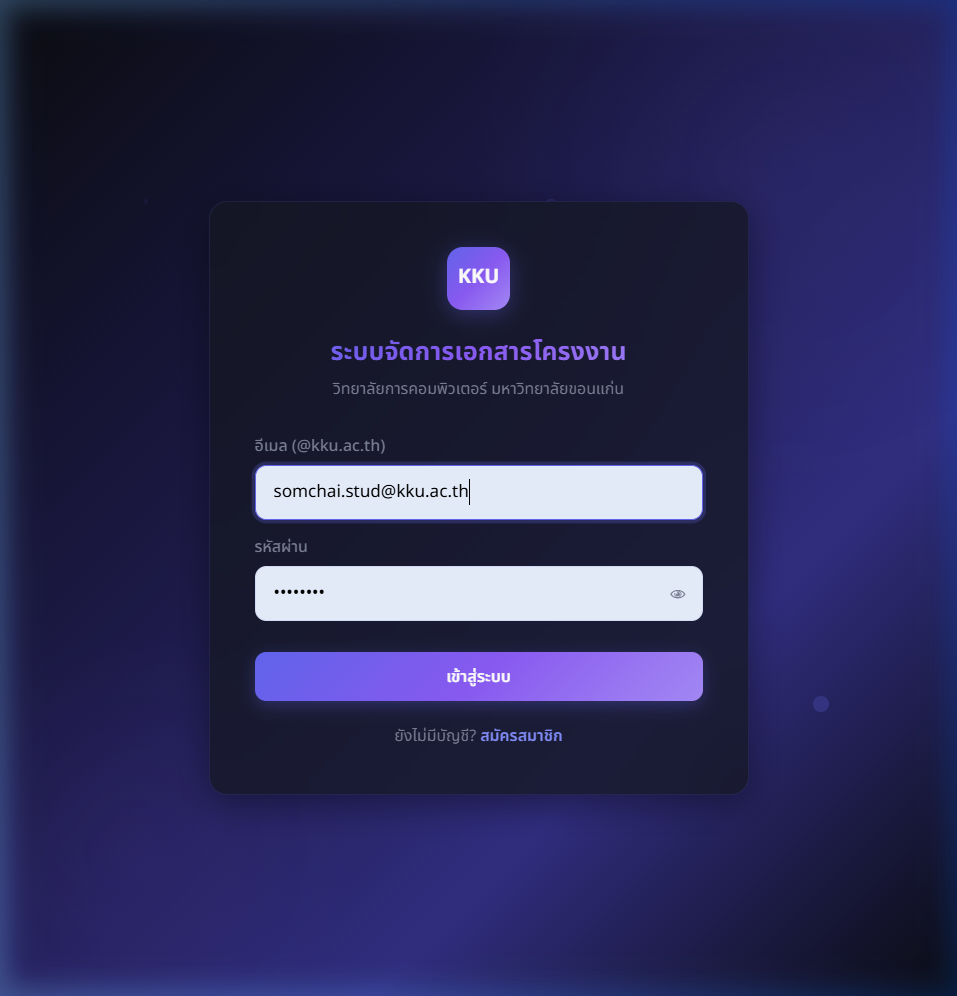
\includegraphics[width=0.8\textwidth]{images/ui-login.png}
\fbox{\parbox{0.75\textwidth}{\centering\vspace{4cm}\textit{แทรกภาพหน้าจอ Login ที่นี่}\\ใช้คำสั่ง \texttt{\textbackslash includegraphics}\vspace{4cm}}}
\caption{หน้าจอเข้าสู่ระบบ (Login)}
\label{fig:ui_login}
\end{figure}

หน้าจอหลัก (Dashboard) แสดงดังภาพที่ \ref{fig:ui_dashboard}

\begin{figure}[H]
\centering
% 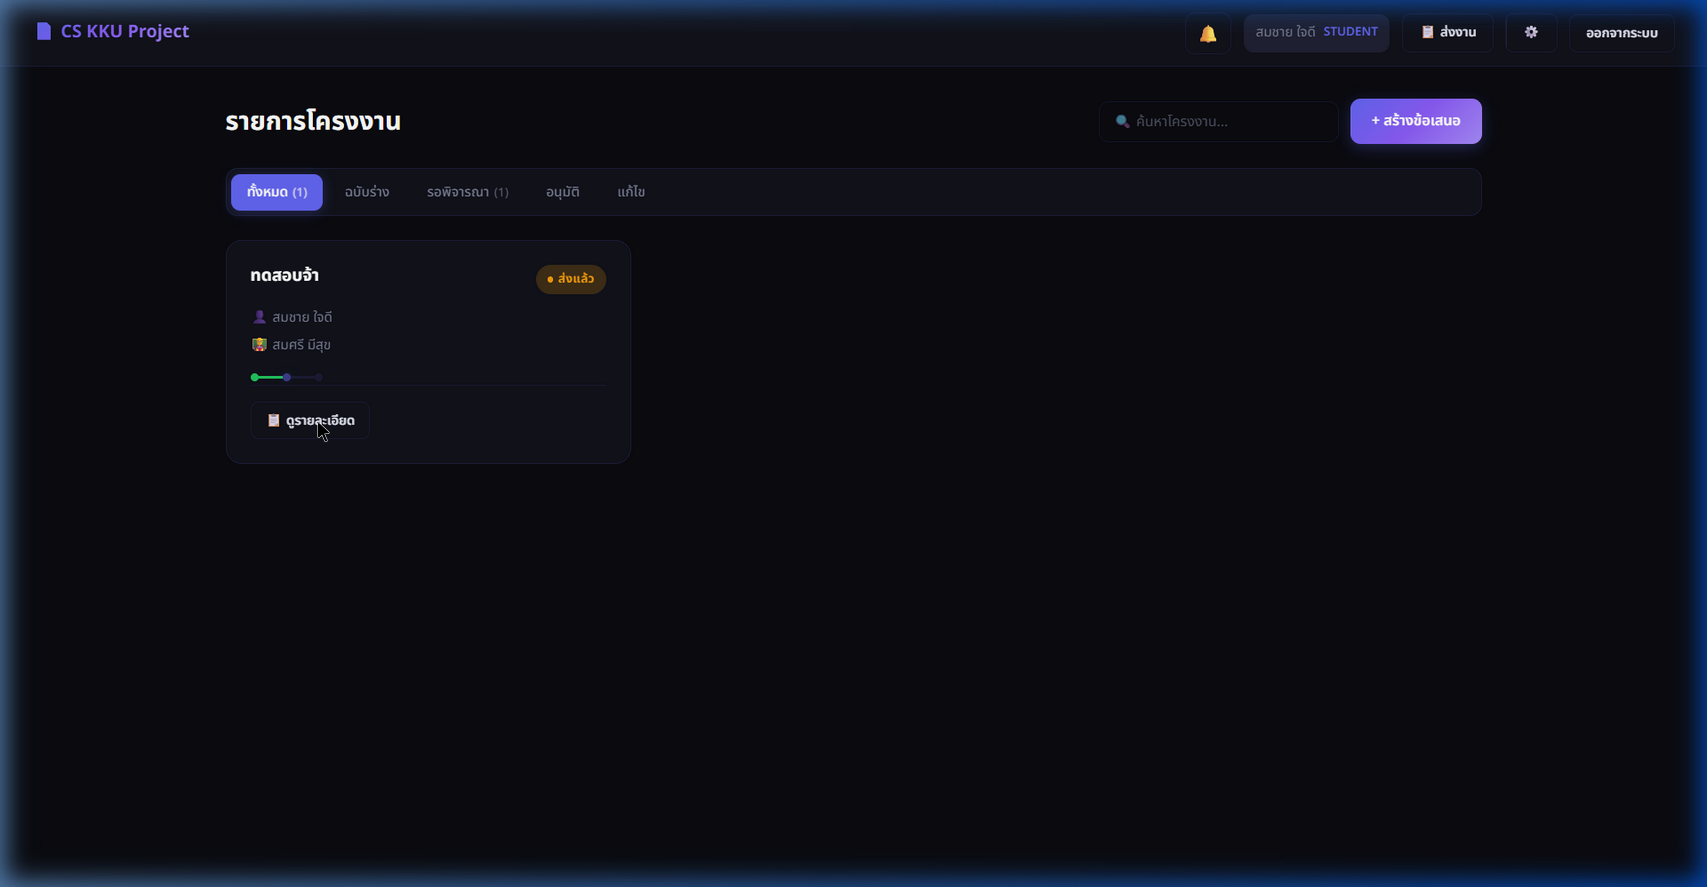
\includegraphics[width=0.8\textwidth]{images/ui-dashboard.png}
\fbox{\parbox{0.75\textwidth}{\centering\vspace{4cm}\textit{แทรกภาพหน้าจอหลักที่นี่}\vspace{4cm}}}
\caption{หน้าจอหลัก (Dashboard)}
\label{fig:ui_dashboard}
\end{figure}

\section*{คู่มือการใช้งาน}

อธิบายขั้นตอนการใช้งานระบบโดยสังเขป\ldots{}

% =============================
% ภาคผนวก ข (ตัวอย่าง — uncomment ถ้าต้องการ)
% =============================
% \appendiceschapter{รายละเอียดเพิ่มเติม}
% \section*{หัวข้อ}
% เนื้อหาภาคผนวก ข
